\chapter{Teoretická část}\label{theoretical}
\section{Charakteristika časových řad}
Časové řady představují posloupnosti datových bodů uspořádaných podle času. 
Jednotlivá pozorování mohou být zaznamenávána v~pravidelných či~nepravidelných časových intervalech nebo mohou být považována za spojitě definovaná v~čase. 
V~případě, že jsou hodnoty měřeny v~konkrétních a~oddělených časových okamžicích, hovoříme o~diskrétní časové řadě. 
Naopak, pokud lze sledovanou veličinu považovat za definovanou v~každém okamžiku času, jedná se o~kontinuální časovou řadu. 
\cite{diggle2025time}

Datové body časových řad mohou reprezentovat širokou škálu jevů, například teplotní záznamy, údaje z~finančních trhů, senzorová měření, dopravní intenzitu nebo spotřebu energie. 
Hodnoty nemusí být nutně číselné, ale mohou být také kategorické, například ve formě stavů zařízení nebo typů událostí. 
Pozorování navíc nemusí odpovídat jedinému časovému okamžiku, ale mohou představovat agregované\footnote{\textit{Agregované} - seskupené} hodnoty za určité časové období, například denní průměrnou teplotu nebo hodinový výkon výrobní linky. 
Délka těchto intervalů závisí na charakteru sledovaného jevu a~požadavcích následné analýzy.
\cite{diggle2025time}

Z~matematického hlediska lze časovou řadu formálně definovat jako množinu pozorování

\begin{equation}
X = \{X_t : t \in T\},
\end{equation}

kde \(X_t\) představuje hodnotu sledované veličiny v~čase \(t\) a~\(T\) je množina časových okamžiků.
\cite{diggle2025time}

\subsection{Analýza}
V~podstatě všechny časové řady jsou zaznamenávány za účelem následné analýzy. Tato analýza může mít různé cíle, které lze shrnout do následujících kategorií:

\begin{itemize}
    \item \textbf{Zkoumání vlivů na sledovaný jev} \\
    Časové řady se často používají k~odhalování vztahů mezi různými faktory a~sledovaným jevem. 
    Například v~ekonomii mohou být analyzovány dopady změn úrokových sazeb na inflaci nebo v~energetice vliv teploty na spotřebu elektrické energie. 
    Taková analýza umožňuje pochopit, jak jednotlivé vlivy ovlivňují chování systému v~čase.
    
    \item \textbf{Zkoumání samotného jevu} \\
    Někdy je cílem zkoumat pouze samotný jev.
    Například meteorologické časové řady teplot mohou odhalit dlouhodobé oteplování, sezónní výkyvy nebo extrémní jevy, jako jsou vlny horka.
    
    \item \textbf{Predikce budoucího vývoje} \\
    Historická data umožňují předpovídat budoucí hodnoty sledovaného jevu. 
    Taková predikce se využívá například při~plánování kapacit výroby, řízení zásob nebo finančních investic.
\end{itemize}

Analýza časových řad zahrnuje různé techniky a~metody, které umožňují identifikovat trendy, sezónnost, závislosti v~čase a~další charakteristiky dat.
\cite{diggle2025time}

\begin{figure}[H]
        \centering
        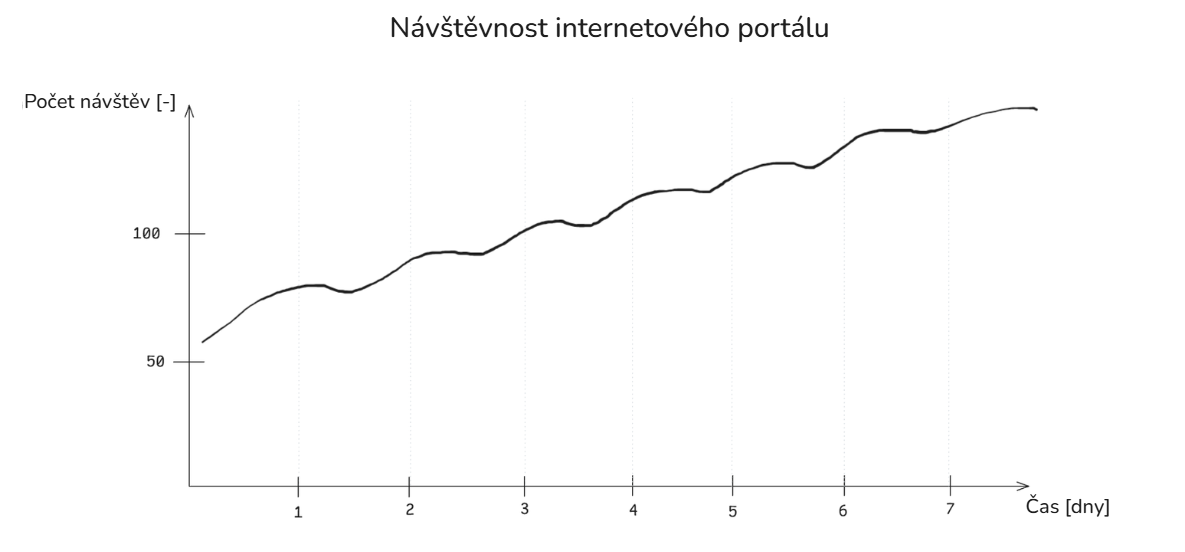
\includegraphics[width=0.8\textwidth]{images/casova_rada.png}
        \caption{Ukázka časové řady (zdroj: vlastní zpracování)}
        \label{fig:casova_rada}
\end{figure}
Na obrázku \ref{fig:casova_rada} je znázorněna ukázka časové řady, kde na vodorovné ose jsou zobrazeny časové okamžiky v~rámci dní a~na svislé ose hodnoty sledovaného jevu - Současných online uživatelů na webovém portálu.

Lze na ní pozorovat denní cyklus, neboli sezónnost, kdy počet uživatelů vrcholí v~odpoledních hodinách a~klesá během noci, a~zároveň lineární rostoucí trend: stránku každý den navštíví více uživatelů.

\section{Ukládání časových řad}
Mnohdy hodnota časových řad leží spíše v~retrospektivní analýze než v~analyzování každé nové hodnoty v~reálném čase.
Z~tohoto důvodu je často potřeba tyto časové řady efektivně ukládat pro pozdější analýzu.
Existuje mnoho různých přístupů k~ukládání časových řad, od tradičních relačních databází přes specializované databázové systémy navržené speciálně pro tento účel až po obyčejné textové soubory.
\cite{nielsen2019practical}
\clearpage
Při~výběru správného formátu a~databázového systému pro ukládání časových řad je důležité zvážit několik faktorů, jako jsou:
\begin{itemize}
    \item \textbf{Objem dat} \\ 
    Časové řady mohou a~mnohdy i~generují daleko větší objemy dat než jiné typy dat. 
    Tento objem je důležité předem odhadnout a~zvolit systém, který je schopný efektivně tento růst zvládnout.
    \cite{kleppmann2017designing}
    
    \item \textbf{Neustálý příjem nebo jednotlivé události} \\
    Při~vybírání ideálního systému, například pro ukládání návštěvnosti webových stránek, je potřeba zvážit charakter dat.  
    V~případě neustálého toku dat je obvykle nejzajímavější pracovat s~nejnovějšími záznamy, protože ty starší mohou být méně relevantní pro analýzu. 
    Naopak pokud data představují jednotlivé události, například každoroční dopravní provoz během svátků, může být důležité mít přístup i~k~historickým datům.
    V~takovém případě je pravděpodobnější, že systém bude potřebovat podporu pro náhodný přístup k~různým časovým intervalům.
    \cite{kleppmann2017designing}
    
    \item \textbf{Trvání projektu} \\
    Pokud je projekt krátkodobý, může být dostačující použít jednodušší a~rychle nasaditelná řešení, jako jsou textové soubory nebo jednoduché databáze.
    Pokud známe délku projektu, daleko snáze se odhaduje objem dat, který bude potřeba uložit.
    \cite{nielsen2019practical}
    
    \item \textbf{Zpracování a~životní cyklus dat} \\ 
    Je vhodné předem stanovit, jak budou data zpracovávána a~jak dlouho mají být uchovávána.  
    Ne všechny záznamy je nutné uchovávat trvale, některé lze po určité době agregovat, downsamplovat\footnote{\textit{Downsampling} - proces převzorkování dat na menší počet datových bodů. \cite{nielsen2019practical}} nebo smazat.  
    Definování jasné strategie mazání či~archivace dat pomáhá předejít nekontrolovatelnému růstu databáze a~zároveň usnadňuje správu a~optimalizaci výkonu systému.  
\end{itemize}    

Tyto faktory také mohou pomoci určit, jestli je nutné ukládat neupravená data nebo předem zpracovaná.

\subsection{Životnost dat}
Při~rozhodování o~tom, jaké úložiště dat je vhodné, je klíčové porozumět životnímu cyklu dat. 
Čím realističtější budeme ohledně skutečného využití dat, tím méně jich je nutné ukládat a~tím méně času strávíme hledáním ideálního úložného systému. 
Mnoho organizací zaznamenává příliš mnoho událostí a~bojí se o~ztrátu dat, ale mít obrovské množství špatně zpracovatelných dat 
je mnohem méně užitečné než mít agregovaná data uložená v~relevantních časových intervalech.

U~krátkodobých dat, například výkonnostních metrik, které se sledují jen kvůli ověření, že je vše v~pořádku, možná vůbec nebude 
potřeba ukládat data v~původní podobě, nebo alespoň ne na dlouho. To je zvlášť důležité u~dat založených na událostech, kde jednotlivé 
události samy o~sobě nejsou významné a~hlavní hodnotu mají až souhrnné statistiky. \cite{nielsen2019practical}

Předpokládejme, že sledujeme dobu načítání webové stránky v~sekundách.
V~tabulce \ref{table:1} je uvedena ukázka časové řady načítání webové stránky v~různých časových okamžicích.
\begin{table}[ht!]
\centering
\begin{tabular}{||c | c||} 
    \hline
    \textbf{Časové razítko} & \textbf{Čas načtení stránky} \\ [0.5ex] 
    \hline\hline
    Duben 5, 2024 10:22:24 & 23s \\ 
    \hline
    Duben 5, 2024 10:22:28 & 15s \\
    \hline
    Duben 5, 2024 10:22:41 & 14s \\
    \hline
    Duben 5, 2024 10:23:02 & 11s \\
    \hline
    Duben 5, 2024 10:23:15 & 19s \\
    \hline
    Duben 5, 2024 10:23:33 & 12s \\
    \hline
\end{tabular}
\caption{Časová řada načítání webové stránky (zdroj: vlastní zpracování)}
\label{table:1}
\end{table}

V~takovém případě nás~nezajímá každý jednotlivý záznam, ale spíše souhrnné statistiky, jako je průměrný čas načítání za minutu, hodinu nebo den.
Proto můžeme zvolit strategii, kde budeme uchovávat pouze agregovaná data, například průměrný čas načítání za každou minutu, a~původní záznamy po určité době smazat.
Tímto způsobem můžeme výrazně snížit objem uložených dat a~zároveň zachovat relevantní informace pro analýzu výkonu webové stránky. \cite{nielsen2019practical}

Výsledný záznam by tedy mohl vypadat například takto v~tabulce \ref{table:2}.
\begin{table}[ht!]
\centering
\begin{tabular}{||c | c | c | c | c||} 
    \hline
    \textbf{Časové rozmezí} & \textbf{Prům. čas načtení} & \textbf{Počet přístupů} & \textbf{Min. čas} & \textbf{Max. čas} \\ [0.5ex] 
    \hline\hline
    Duben 5, 2024 10:00:00 & 15.6s & 6 & 11s & 19s \\ 
    \hline
    Duben 5, 2024 11:00:00 & 17.2s & 4 & 9s & 25s \\
    \hline
\end{tabular}
\caption{Zjednodušený záznam načítání webové stránky (zdroj: vlastní zpracování)}
\label{table:2}
\end{table}

\section{Databázové systémy}
Databázové systémy jsou ten nejběžnější způsob, jak ukládat časové řady.  Většinou jsou připravené tzv. "out of the box", neboli ihned po pořízení, 
poskytují spoustu vestavěných funkcí pro jednoduché zpracování dat, jako je například agregace a~filtrování.
Navíc jsou optimalizované pro rychlý zápis a~čtení dat, a~dokáží škálovat s~rostoucím objemem dat. \cite{nielsen2019practical}

\subsection{OLTP a~OLAP databáze}

Databázové systémy lze rozdělit podle typu pracovního zatížení na systémy OLTP (Online Transaction Processing) a~OLAP (Online Analytical Processing). 
Oba přístupy jsou navrženy pro odlišné způsoby práce s~daty a~liší se zejména charakterem dotazů, způsobem ukládání dat a~optimalizací výkonu. 
\cite{clickhouseoltpvsolap}

\begin{itemize}
    \item \textbf{OLTP} \\
    OLTP databáze jsou určeny pro každodenní provoz aplikací, kde probíhá velké množství krátkých transakcí, například vkládání, aktualizace nebo mazání jednotlivých záznamů. 
    Typickými příklady jsou bankovní systémy, rezervační systémy nebo e-shopy. 
    Tyto databáze jsou optimalizovány především pro rychlé zápisy a~čtení jednotlivých řádků při~zachování konzistence dat pomocí ACID\footnote{\textit{ACID} označuje čtyři~vlastnosti databázových transakcí – atomičnost, konzistenci, izolaci a~trvalost – které zajišťují správné a~spolehlivé zpracování dat. \cite{mongodbacid}} transakcí.
    \cite{clickhouseoltpvsolap}

    \item \textbf{OLAP} \\
    OLAP databáze jsou určeny pro analytické zpracování velkého objemu historických dat. 
    Místo jednotlivých záznamů pracují s~rozsáhlými datovými sadami a~jsou optimalizovány pro agregace, filtrování a~statistické analýzy. 
    Typickými příklady využití jsou business intelligence, reporting nebo analýza časových řad. 
    Často využívají sloupcové ukládání dat, které umožňuje efektivně zpracovávat dotazy nad miliony až miliardami záznamů.
    \cite{clickhouseoltpvsolap}
\end{itemize}

Databáze určené pro ukládání časových řad často kombinují vlastnosti obou přístupů. 
Musí zvládat vysokou rychlost zápisu nových měření podobně jako OLTP databáze, současně však umožňují rychlé analytické dotazy nad historickými daty, které jsou charakteristické pro OLAP systémy.
\cite{clickhouseoltpvsolap}

\subsection{SQL a~NoSQL databáze}
Dále lze databázové systémy rozdělit z~hlediska datového modelu na dvě hlavní skupiny, relační (SQL) a~nerelační (NoSQL) databáze. 
Relační databáze ukládají data do tabulek propojených vzájemnými vztahy a~využívají standardizovaný jazyk SQL (Structured Query Language). 
Naproti tomu NoSQL databáze nejsou založeny na relačním modelu a~nabízejí různé způsoby organizace dat podle požadavků konkrétní aplikace.

Hlavní rozdíly mezi oběma přístupy spočívají zejména ve způsobu organizace dat a~flexibilitě datového modelu. \cite{microsoftnosql}
\begin{itemize}
    \item \textbf{SQL} \\
    Relační databáze používají pevně definované schéma, takže každá tabulka má předem určené sloupce a~jejich datové typy.
    Tento přístup zajišťuje vysokou konzistenci dat a~je vhodný zejména v~případech, kdy je struktura dat předem známá a~v~průběhu času se výrazně nemění. 
    \cite{microsoftsql}
    \begin{figure}[H]
        \centering
        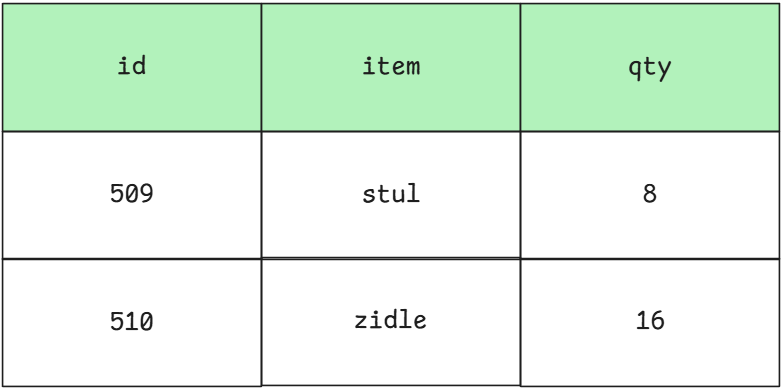
\includegraphics[width=0.4\textwidth]{images/sql_example.png}
        \caption{Ukázka struktury SQL tabulky (zdroj: Vlastní zpracování)}
        \label{fig:sql_example}
    \end{figure}
    \item \textbf{NoSQL} \\ 
    NoSQL databáze nejsou omezeny pevným schématem, což umožňuje jednodušší přizpůsobení měnící se struktuře dat.
    Podle způsobu organizace dat je lze rozdělit do několika kategorií, z~nichž nejčastější jsou:
    \begin{itemize}
        \item \textbf{Databáze párů klíč-hodnota} \\ 
        Ukládají data jako páry klíč-hodnota, což umožňuje rychlý přístup k~záznamům na základě klíče. 
        Jsou vhodné zejména tam, kde je známý identifikátor záznamu, zatímco samotná hodnota může mít různou strukturu. Takové databáze zpravidla nedokáží například přes hodnoty filtrovat, ale zato je dokáží najít konstatní časové složitosti, úkol zabere vždy stejný časv~(O(1)).

        Typickým představitelem je Redis, který je často využíván pro 
        caching\footnote{\textit{Caching} - technika ukládání často používaných dat do rychlé paměti} a~real-time aplikace jakožto 
        dodatečná vrstva mezi uživatelem a~koncovou databází. \cite{redisusecases}
        
        \begin{figure}[H]
            \centering
            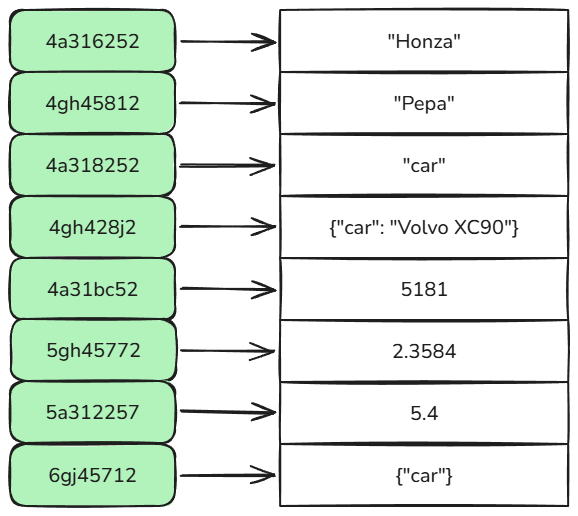
\includegraphics[width=0.5\textwidth]{images/key_value.png}
            \caption{Ukázka struktury databáze párů klíč-hodnota (zdroj: vlastní zpracování)}
            \label{fig:key_value_example}
        \end{figure}
        \item \textbf{Dokumentová databáze} \\ 
        Ukládají data ve formě dokumentů, často ve formátu JSON\footnote{\textit{JSON} - textový formát pro ukládání a výměnu strukturovaných dat}\footnote{https://www.json.org/json-en.html}~(JavaScript Object Notation) nebo BSON~(Binary JSON)\footnote{\textit{BSON} - binární obdoba JSON s podporou dalších datových typů}\footnote{https://bsonspec.org}. 
        Jednotlivé dokumenty mohou mít odlišnou strukturu a~bývají sdružovány do kolekcí.
        Díky podpoře vnořených objektů jsou vhodné pro aplikace, u~nichž se datový model často mění. Velmi dobře dokáží zpracovat právě například strukturu JSONu, takže se nimi dá například velmi snadno filtrovat.

        Typickým představitelem je MongoDB. Často se používá pro webové aplikace, analytické systémy nebo logování, kde se struktura dat může často měnit. \cite{mongodbusecases}
        \begin{figure}[H]
            \centering
            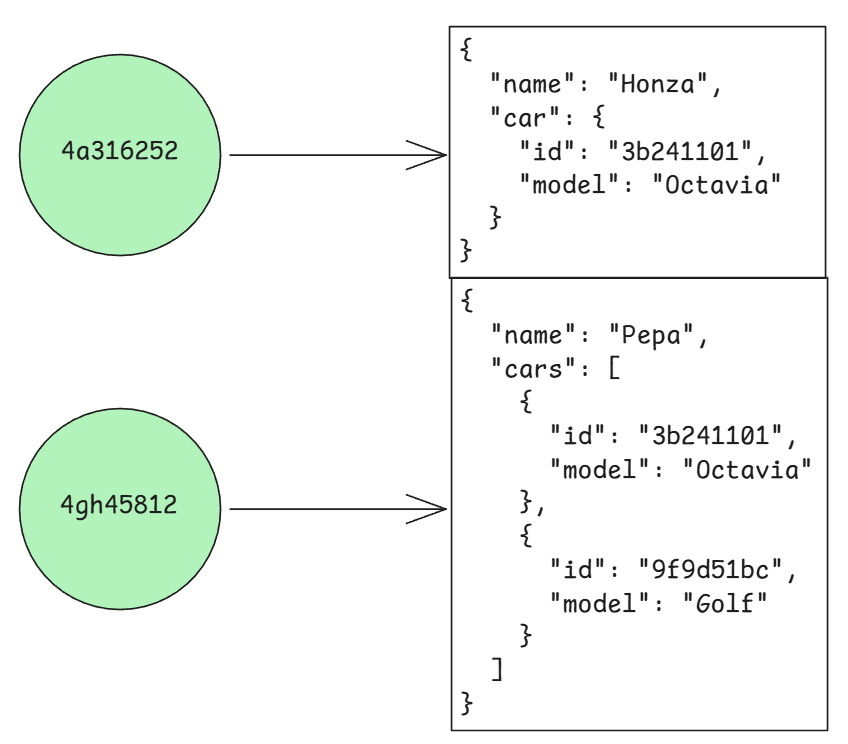
\includegraphics[width=0.6\textwidth]{images/document.png}
            \caption{Ukázka struktury dokumentové databáze (zdroj: vlastní zpracování)}
            \label{fig:document_example}
        \end{figure}
        \item \textbf{Sloupcové databáze} \\ 
        Ukládají data po sloupcích namísto řádků, což je výhodné zejména při~analytických dotazech, pracujících pouze s~vybranými atributy.
        Omezením čtení pouze potřebných sloupců se snižuje objem načítaných dat a~zvyšuje výkon analytických operací.

        Typickým představitelem je ClickHouse, který je často využíván pro analytické úlohy v~reálném čase, jako je sledování metrik a~logování. \cite{clickhouseusecases}
        \begin{figure}[H]
            \centering
            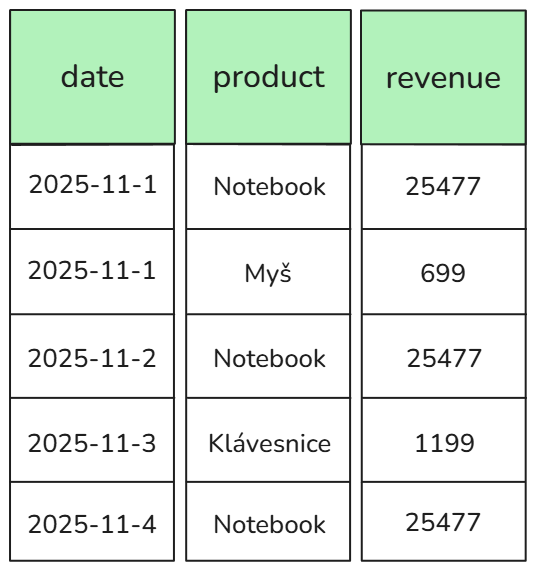
\includegraphics[width=0.55\textwidth]{images/columnar.png}
            \caption{Ukázka struktury sloupcové databáze (zdroj: vlastní zpracování)}
            \label{fig:columnar_example}
        \end{figure}

        \item \textbf{Grafová databáze} \\ 
        Ukládají data ve formě uzlů a~hran reprezentujících vzájemné vztahy mezi entitami.
        Jsou vhodné především pro úlohy, kde jsou vztahy mezi objekty důležitější než samotné atributy objektů.

        Typickým představitelem je Neo4j\footnote{https://neo4j.com}, který se často používá pro sociální sítě, doporučovací systémy a~analýzu podvodů. \cite{neo4jusecases}
        \begin{figure}[H]
            \centering
            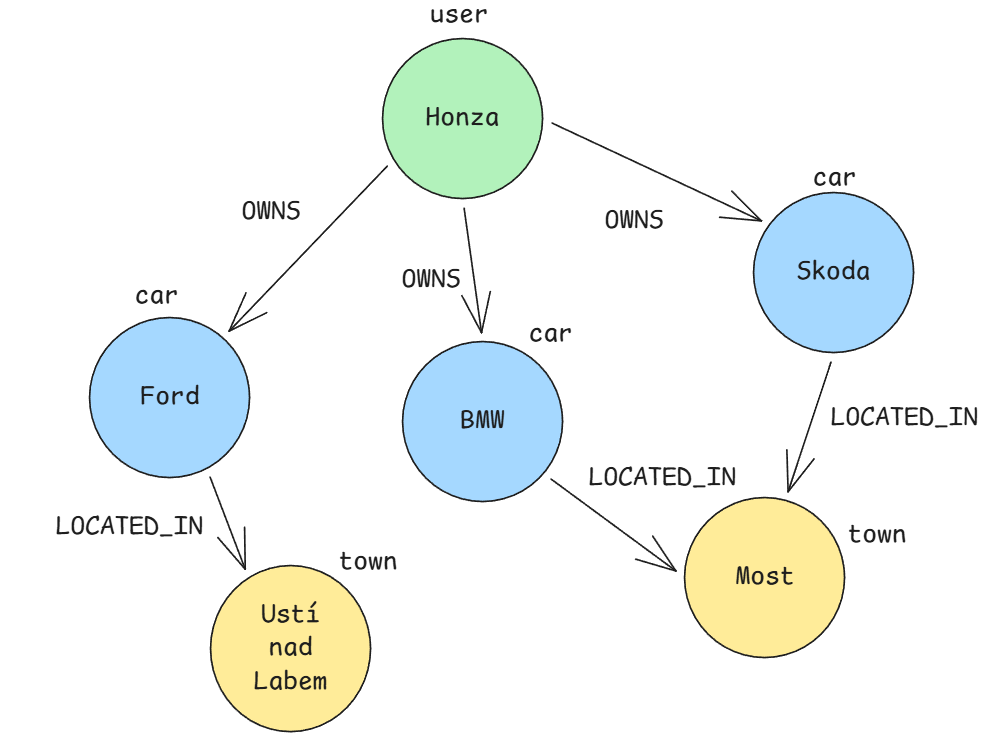
\includegraphics[width=0.6\textwidth]{images/graph_example.png}
            \caption{Ukázka struktury grafové databáze (zdroj: vlastní zpracování)}
            \label{fig:graph_example}
        \end{figure}
    \end{itemize}
\end{itemize}

\subsection{Datové struktury}
Databázové systémy se liší nejen způsobem organizace dat, ale také vnitřními datovými strukturami, které používají pro ukládání a~vyhledávání záznamů.
Mezi ty nejběžnější patří B-Tree a~LSM strom.
Tyto struktury výrazně ovlivňují výkon databázového systému a~určují, jak následně co nejefektivněji daný databázový systém využít.

\subsubsection{B-Tree}\label{btree}
B-Tree je datová struktura, která uchovává data ve formě klíč-hodnota, která jsou seřazené podle klíče.

B-Tree rozdělí úložiště dat do několika fixních bloků (často odpovídajících velikosti diskového sektoru).
Každý takový blok může být lehce identifikovaný pomocí adresy a~jeden blok může obsahovat více adres odkazujících na jiné bloky. \cite{kleppmann2017designing}
Jeden blok je označený za kořenový blok, který je vždy výchozím bodem pro hledání dat.

\begin{figure}[H]
    \centering
    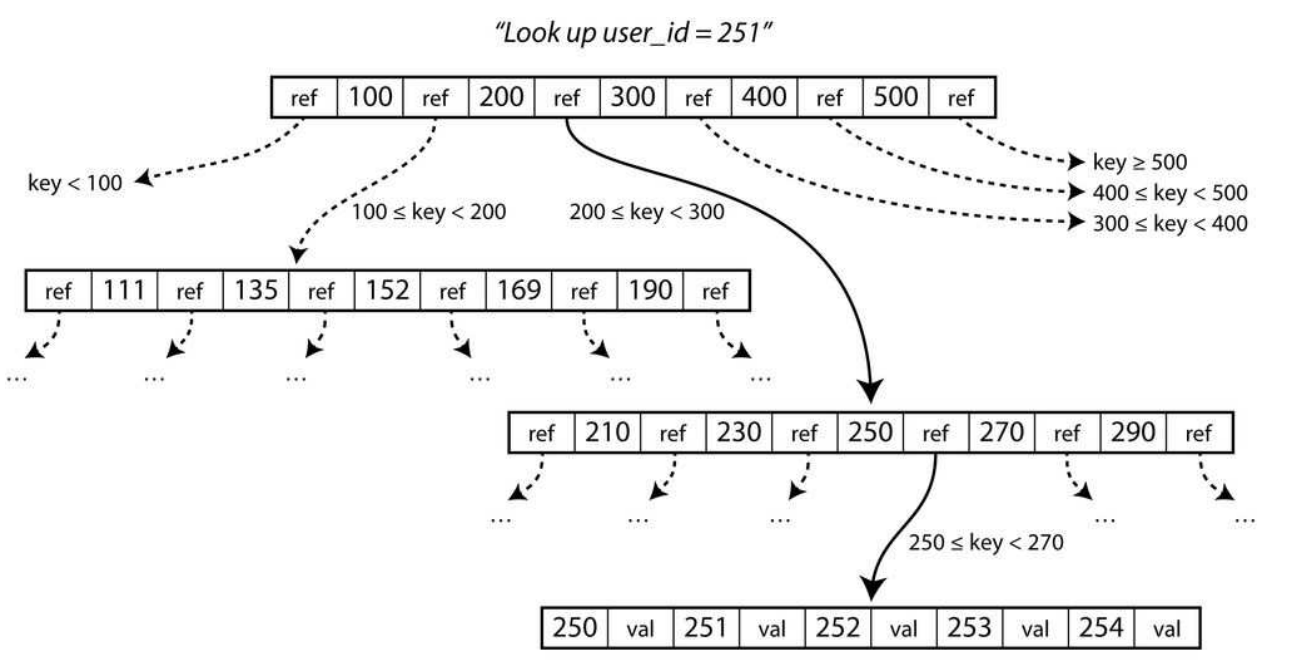
\includegraphics[width=0.8\textwidth]{images/b-tree_example.png}
    \caption{Ukázka organizace dat v~B-Tree struktuře (převzato z~\cite{kleppmann2017designing})}
    \label{fig:btree}
\end{figure}

V~ukázce na obrázku \ref{fig:btree} hledáme záznam s~klíčem 251, takže víme, že musíme sledovat odkaz do seznamu 200-299.
Takový seznam se dále dělí do bloků seřazené od 200-209, 210-229, 230-249, 250-269, 270-289 a~290-29x.
Eventuelně se dostaneme až do správného bloku, který hledáme. 
\cite{kleppmann2017designing}

\subsubsection{LSM Strom}\label{lsm_tree}
Log-Structured Merge-Tree je datová struktura optimalizovaná pro vysokou propustnost zápisů.
Každý zápis se nejprve uloží do rychlé paměti (memtable) a~periodicky se přepíše do trvalého úložiště (disku) ve formě seřazených souborů (SSTables).
Tyto SSTables jsou přirozené seřazené podle klíče a~jsou už dále neměnné. \cite{kleppmann2017designing}

Při~čtení se pak postupuje nejdříve přečtením memtables a~následně od nejnovějších SSTables k~nejdřívějším, dokud se nenajde požadovaný záznam nebo se nedojde na konec. \cite{kleppmann2017designing}

\begin{figure}[H]
    \centering
    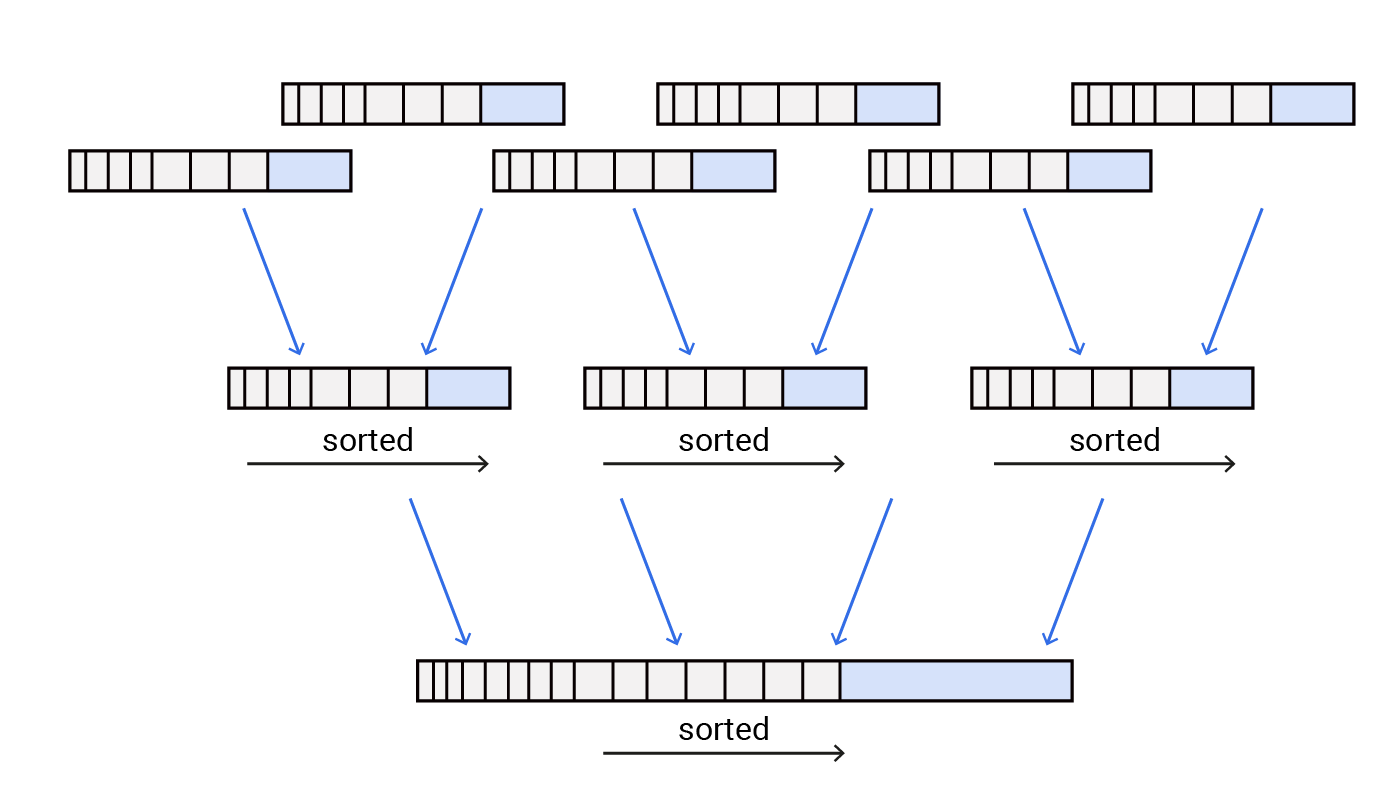
\includegraphics[width=0.8\textwidth]{images/lsmtree_example.png}
    \caption{Ukázka organizace dat v~LSM stromu (převzato z~\cite{lsmtree})}
    \label{fig:lsmtree}
\end{figure}

Starší SSTables jsou pravidelně slučovány do větších souborů, aby se snížil počet souborů, které je třeba prohledávat při~čtení, a~aby se odstranily záznamy, které byly aktualizovány nebo smazány.
Díky tomu že jsou přirozeně seřazené, je tento proces slučování efektivní. \cite{kleppmann2017designing}

\section{Úvod do problematiky testování a~implementace}
Při~porovnávání databázových systémů je důležité zajistit, aby byly všechny testy prováděny ve srovnatelných podmínkách. 
Rozdíly v~konfiguraci serverů, nainstalovaném softwaru nebo způsobu nasazení mohou výrazně ovlivnit dosažené výsledky a~vést ke zkresleným závěrům. 
Proto je vhodné využívat izolovaná a~snadno reprodukovatelná prostředí, ve kterých lze jednotlivé systémy nasazovat opakovaně a~konzistentně.

Taková prostředí dělíme na dva hlavní typy: kontejnery a virtuální stroje.
\begin{figure}[H]
    \centering
    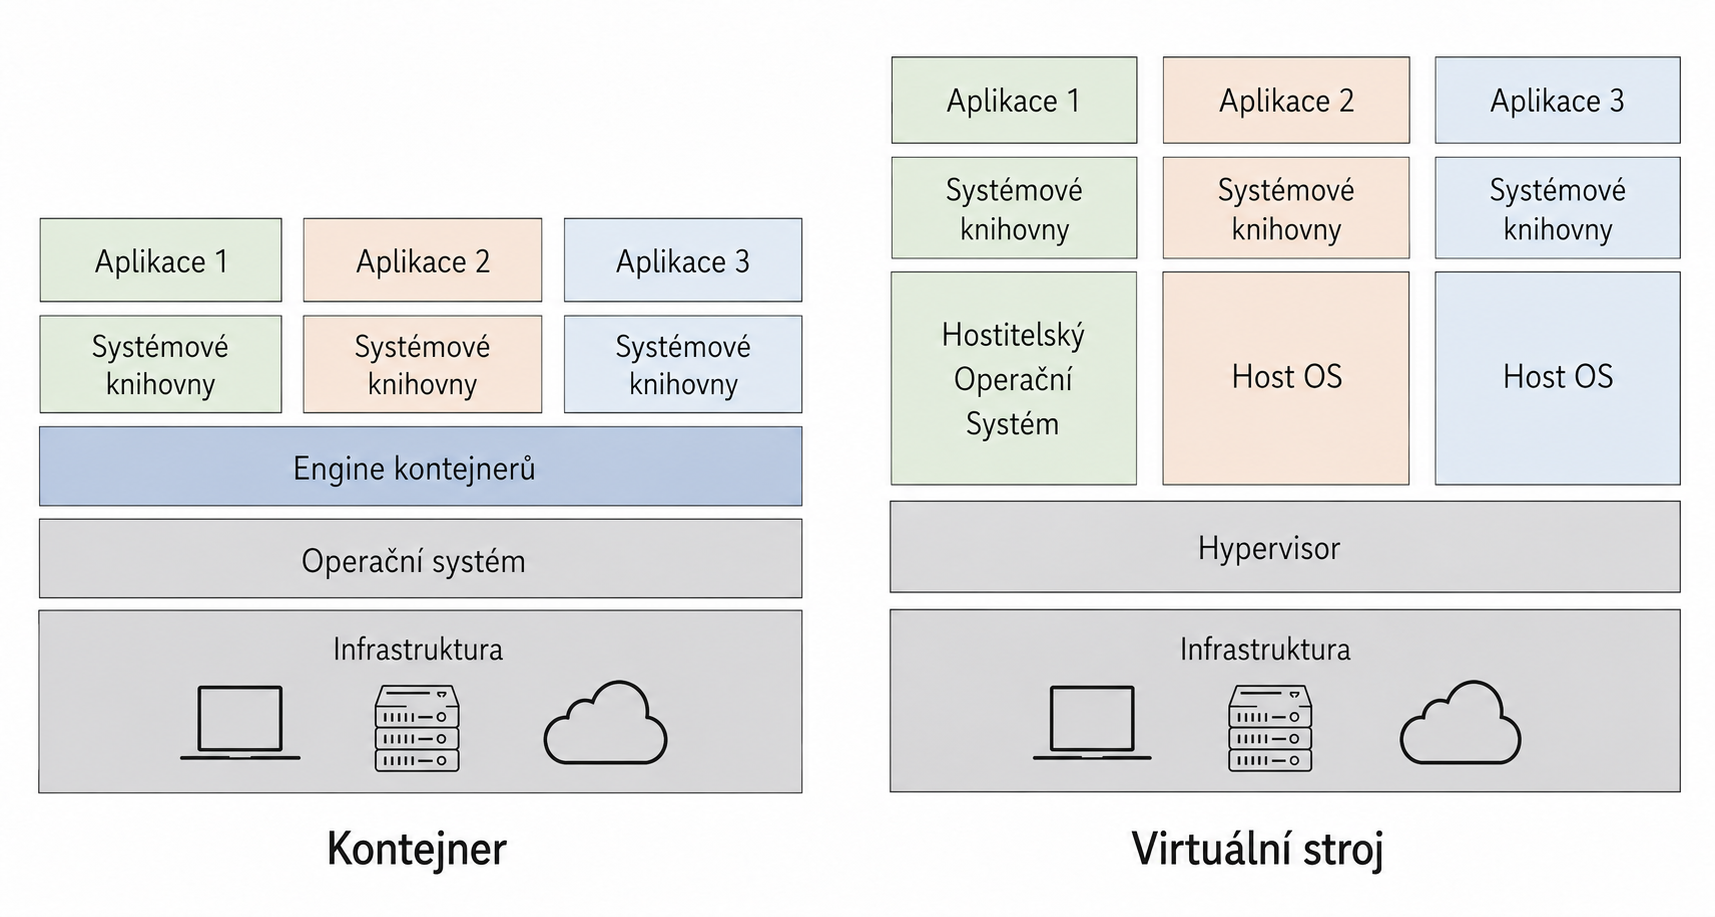
\includegraphics[width=0.8\textwidth]{images/vmvscontainer.png}
    \caption{Kontejner a~virtuální zdroj (zdroj: vlastní zpracování)}
    \label{fig:vmvscontainer}
\end{figure}


\subsection{Kontejner}
Kontejner představuje standardizovanou softwarovou jednotku, která zapouzdřuje kód aplikace společně se všemi jejími závislostmi a~knihovnami. 
Na rozdíl od virtuálních strojů kontejnery neobsahují vlastní operační systém a~nevyužívají hypervizor. 
Místo toho sdílejí jádro hostitelského systému, což zajišťuje izolaci procesů při~zachování minimální režie. 
Díky tomu jsou kontejnery výrazně menší (často v~řádech megabajtů) a~jejich spuštění je rychlejší. \cite{redhatcontainers}

Klíčovou vlastností kontejnerů je jejich přenositelnost. Aplikaci zabalenou v~kontejneru lze snadno přesouvat mezi různými 
prostředími, ať už od lokálního vývoje až po produkční nasazení v~cloudu, s~jistotou, že bude fungovat konzistentně bez ohledu na podkladovou 
infrastrukturu. O~masivní rozšíření a~standardizaci této technologie se v~posledních letech zasloužila především platforma Docker.

\subsection{Virtuální stroj}
Virtuální stroj je softwarová emulace fyzického počítače, která spouští vlastní kompletní operační systém v~izolovaném prostředí. 
Provoz více virtuálních strojů na jednom fyzickém serveru umožňuje vrstva zvaná hypervizor, která se stará o~přidělování 
hardwarových prostředků (CPU, paměť, úložiště) jednotlivým instancím. \cite{redhatcontainers}

Hypervizory lze rozdělit do dvou hlavních kategorií:


\begin{itemize}
    \item \textbf{Bare-metal} \\
    Také nazývaný Type 1, běží přímo na fyzickém hardwaru hostitelského serveru bez prostřednictví operačního systému. Díky přímému přístupu k~hardwarovým 
    prostředkům je velmi efektivní a~nabízí vysoký výkon, což z~něj činí standardní volbu pro podniková datová centra a~cloudová prostředí. 
    Mezi známé zástupce patří VMware ESXi, Microsoft Hyper-V~nebo KVM (Kernel-based Virtual Machine), který je součástí jádra Linuxu. 
    \cite{redhathypervisors}

    \item \textbf{Hosted} \\
    Také nazývaný Type 2, instaluje se jako běžná softwarová aplikace na již existující operační systém (tzv. hostitelský OS). Hardwarové zdroje jsou 
    virtuálním strojům přidělovány prostřednictvím tohoto hostitelského systému, což zvyšuje režii a~mírně snižuje výkon. Tento 
    typ se nejčastěji využívá na osobních počítačích pro vývoj, testování nebo výuku. Typickými příklady jsou Oracle VirtualBox nebo VMware Workstation.
    
    Infrastrukturou může připomínat kontejner, protože i~on potřebuje ke svému běhu hostitelský operační systém. 
    Zásadní rozdíl však spočívá v~úrovni virtualizace: zatímco kontejner sdílí jádro hostitelského OS a~izoluje pouze uživatelský prostor, Type 2 hypervisor virtualizuje celý hardware a~umožňuje běh úplně samostatných operačních systémů s~vlastními jádry.
    \cite{redhathypervisors}
\end{itemize}
\begin{figure}[H]
    \centering
    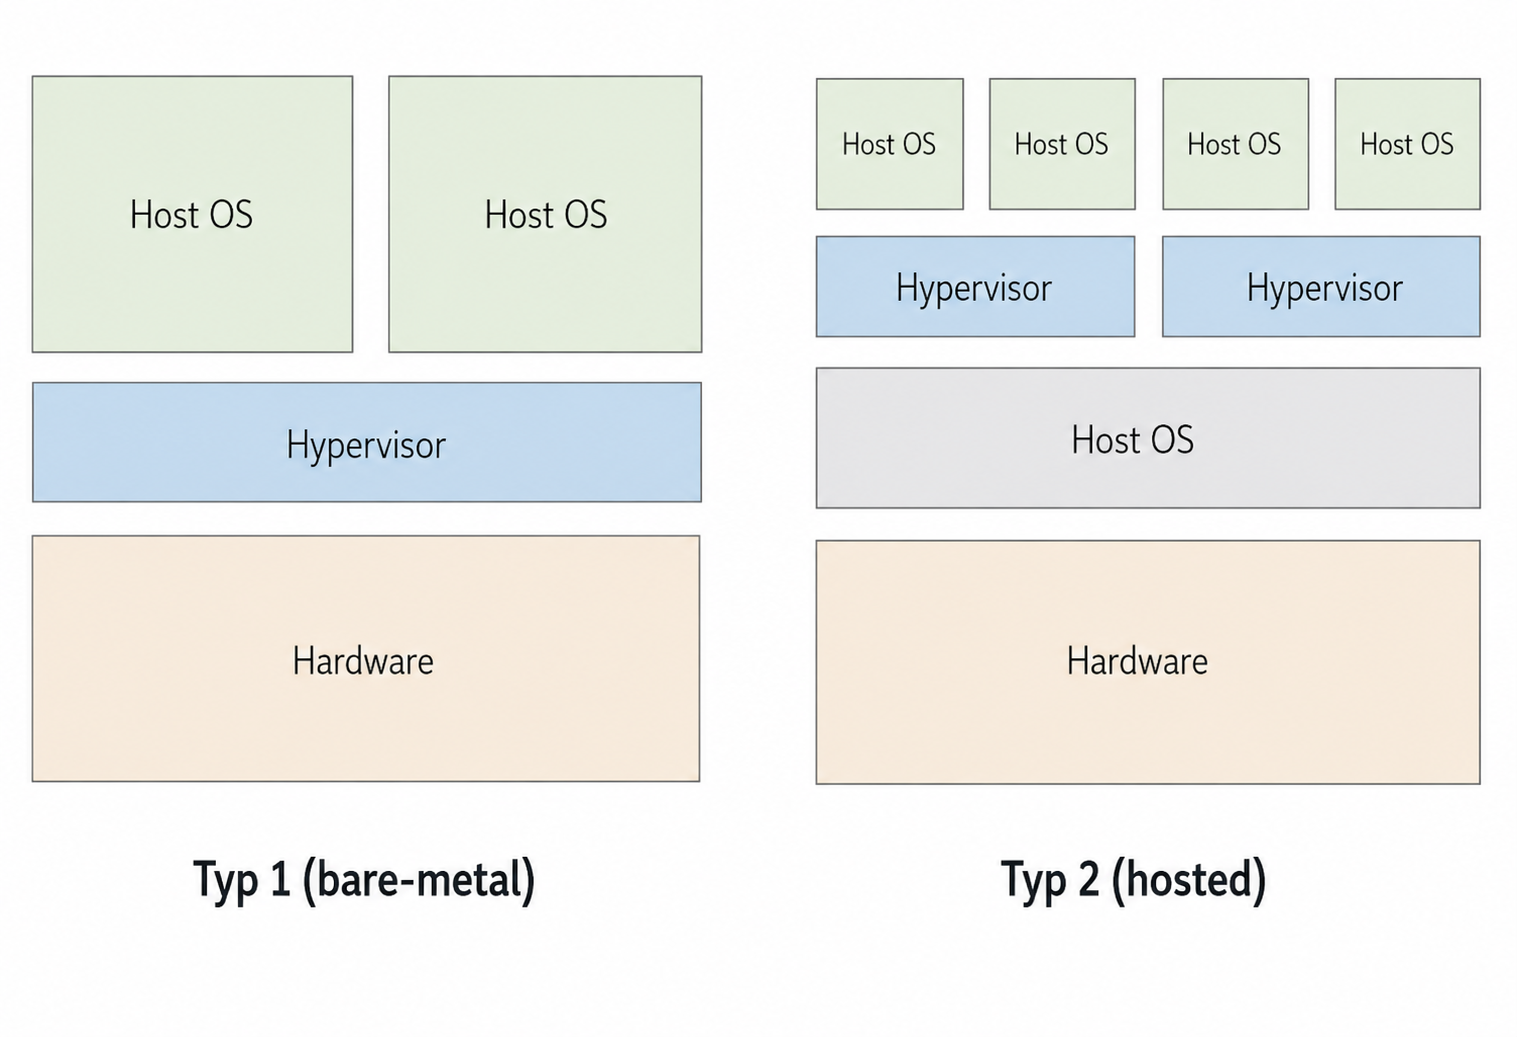
\includegraphics[width=0.75\textwidth]{images/vmtypes.png}
    \caption{Porovnání Typu 1 a~Typu 2 hypervizorů (zdroj: vlastní zpracování)}
    \label{fig:vmtypes}
\end{figure}

\subsection{Zástupce kontejneru - Docker}
Docker je open-source platforma, která v~roce 2013 výrazně popularizovala technologii kontejnerizace a~stala se de facto standardem pro balení, distribuci a~spouštění aplikačních kontejnerů. 
Jádrem ekosystému je Docker Engine, démon\footnote{\textit{Démon (Daemon)} - program běžící na pozadí OS, který automaticky provádí určité úlohy nebo poskytuje služby bez přímé interakce uživatele} běžící na hostitelském operačním systému, který využívá funkcí jádra Linuxu k~vytváření a~správě izolovaných kontejnerů. 
Aplikace je definována deklarativně v~souboru nazvaném Dockerfile, který popisuje základní obraz (base image), závislosti, konfiguraci prostředí a~způsob spuštění aplikace. 
Výsledný obraz je poté přenosný a~může být dále distribuován, přičemž nejznámějším veřejným registrem je Docker Hub. 
\cite{dockerdocs}

\subsection{Zástupce virtuálního stroje typu bare-metal - LXD}
LXD je moderní nástroj pro správu systémových kontejnerů a~virtuálních strojů. 
LXD umožňuje provozovat kompletní linuxové systémy v~izolovaných prostředích. 
Podporuje širokou škálu linuxových distribucí a~nabízí jednotné rozhraní pro jejich spouštění a~správu. 
LXD je navržen tak, aby byl použitelný jak na jediném počítači, tak v~rozsáhlých clusterech\footnote{\textit{Cluster} – skupina propojených serverů pracujících jako jeden logický celek} v~datových centrech. 
Díky tomu se hodí jak pro vývojářská prostředí, tak pro produkční nasazení. 
Mezi jeho praktické funkce patří například snímky stavu kontejnerů, přesun běžících instancí mezi servery nebo integrovaná správa úložiště a~sítí. 
\cite{lxddocs}

\subsubsection{LXC jako základní technologie}

LXD interně staví na technologii LXC (Linux Containers), která přímo využívá funkcí linuxového jádra pro izolaci procesů. 
Zatímco LXC poskytuje nízkoúrovňové nástroje pro vytváření kontejnerů, LXD tyto možnosti obaluje do přehledného REST API\footnote{\textit{API} - Application Programming Interface, rozhraní, přes které spolu komunikují různé aplikace} a~přidává pokročilé funkce pro správu. 
V~praxi to znamená, že LXD neimplementuje vlastní mechanismy virtualizace, ale rozšiřuje osvědčené základy LXC o~moderní způsob ovládání a~orchestrace. \cite{lxcintro}

\subsection{Zástupce virtuálního stroje typu hosted - VirtualBox}
Oracle VM VirtualBox je multiplatformní virtualizační software, který umožňuje provoz více virtuálních strojů s~různými operačními systémy (hostovanými systémy) na jednom fyzickém počítači. 
Podporuje širokou škálu hostitelských platforem včetně Windows, macOS a~Linux, což z~něj činí univerzální nástroj pro vývojáře, testery i~výukové účely. 
Mezi klíčové funkce patří podpora snapshotů (uložení stavu virtuálního stroje pro pozdější návrat), virtuální sítě různých typů (NAT, bridge, internal network) a~dynamické přidělování úložného prostoru. 
I~přes praktickou všestrannost je třeba mít na zřeteli, že VirtualBox běží jako aplikace nad hostitelským OS, čímž vzniká dodatečná výkonnostní režie při~přístupu k~hardwarovým prostředkům, zejména v~oblasti grafického výstupu a~síťové komunikace. \cite{virtualboxdocs}

\subsection{Automatizace přípravy prostředí}
Ruční vytváření takových prostředí je časově náročné a~s~rostoucím počtem testovaných systémů také náchylné k~chybám. 
Z~tohoto důvodu se v~současnosti právě běžně využívají technologie virtualizace a~kontejnerizace společně s~nástroji pro automatizaci konfigurace. 
Ty umožňují připravit nové testovací prostředí během několika minut a~zajistit, že bude nakonfigurováno stejným způsobem při~každém spuštění testu.

Důležitou součástí tohoto přístupu je také koncept Infrastructure as Code, kdy je konfigurace infrastruktury popsána pomocí textových souborů a~může být verzována stejně jako zdrojový kód aplikace. 
Díky tomu lze celý proces nasazení jednoduše opakovat, upravovat a~sdílet mezi různými prostředími.

\subsubsection{Agent a~agent-less přístup}
Při~automatizaci přípravy prostředí lze rozlišit dva základní přístupy ke správě cílových uzlů: \textit{agent-based} (založený na agentech) a~\textit{agent-less} (bez agentů). 
Volba mezi nimi závisí na charakteru spravované infrastruktury, požadavcích na spolehlivost a~frekvenci změn konfigurace.
\begin{itemize}
    \item \textbf{Agent-based přístup} \\
    Tento přístup vyžaduje instalaci speciálního softwaru, tzv. agenta, na každý cílový uzel.
    Agent pravidelně komunikuje s~centrálním řídicím serverem, přijímá deklarativní definici požadovaného stavu systému a~kontinuálně zajišťuje, že skutečná konfigurace uzlu odpovídá tomuto definovanému stavu. 
    Díky lokálně běžícímu procesu dokáže agent automaticky detekovat a~napravit změny v~konfigurace i~během výpadku síťového spojení, neboť není závislý na permanentní dostupnosti řídicího serveru.
    \cite{puppetagent}

    Tento model je proto především vhodný pro dlouhodobě existující systémy v~produkčním prostředí, kde je klíčová spolehlivost. 
    Nevýhodou je vyšší počáteční režie spojená s~nasazením, aktualizací a~zabezpečením agentů na každém cílovém zařízení. 
    \cite{puppetagent}
    \item \textbf{Agent-less přístup} \\
    Agent-less přístup nevyžaduje instalaci žádného permanentního softwaru na cílových uzlech. 
    Řídicí stroj se k~nim připojí standardními bezpečnými protokoly, typicky SSH\footnote{\textit{SSH} - protokol pro bezpečnou komunikaci mezi uzly}, přenese dočasný skript či~modul, který se vykoná lokálně na cílovém uzlu, a~poté se spojení ukončí. 
    \cite{puppetagent}

    Tento model výrazně zjednodušuje počáteční nasazení a~snižuje režii na cílových uzlech, protože není nutné spravovat žádnou stálou infrastrukturu agentů. 
    Na druhou stranu neposkytuje průběžné sledování stavu. 
    Konfigurace se aplikuje pouze na vyžádání při~explicitním spuštění, a~pokud dojde k~nežádoucím změnám, neexistuje agent, který by je automaticky detekoval a~napravil. 
    Agent-less nástroje proto často používají task-based model, kdy je postupně vykonávána předem definovaná posloupnost kroků, nikoli deklarativní popis cílového stavu. 
    \cite{puppetagent}
\end{itemize}


\renewcommand{\arraystretch}{1.5}
\begin{table}[h]
\centering
\begin{tabular}{|
>{\raggedright\arraybackslash}p{3.5cm}|
>{\raggedright\arraybackslash}p{5.5cm}|
>{\raggedright\arraybackslash}p{5.5cm}|}
\hline
\textbf{Kritérium} & \textbf{Agent-based} & \textbf{Agent-less} \\
\hline
Nasazení & Instalace a~registrace agenta na každý uzel & Žádná předchozí příprava uzlu není nutná \\
\hline
Režie na uzlu & Stálý běh agenta (CPU, paměť, síťová komunikace) & Pouze dočasná během provádění úlohy \\
\hline
Model správy & Definovaný cílový stav & Seznam úloh \\
\hline
Spolehlivost při~výpadku & Lokální stav, následná synchronizace & Vyžaduje síťové spojení a~přístupová práva \\
\hline
\end{tabular}
\renewcommand{\arraystretch}{1}
\caption{Srovnání agent-based a~agent-less přístupu (zdroj: vlastní zpracování)}
\label{tab:agent}
\end{table}

Dostupné nástroje ovšem nejsou striktně omezeny na jeden z~těchto přístupů.
Velmi často různě kombinují obě strategie, aby vyhověly specifickým potřebám spravované infrastruktury.

Jako hlavní představitele agent-based nástrojů lze uvést Puppet, zatímco mezi agent-less nástroje patří Ansible.
Přestože se jednotlivé nástroje liší svou architekturou a~způsobem komunikace s~cílovými uzly, sdílejí několik společných principů, které tvoří základ moderní automatizace konfigurací:

\begin{itemize}
\item \textbf{Idempotence} \\
Opakované spuštění stejné konfigurace by mělo vést ke stejnému výsledku, aniž by docházelo k~dalším změnám, pokud je systém již v~požadovaném stavu. 
Tento princip zajišťuje bezpečnost a~předvídatelnost automatizace. 
Ve specifických případech, například při~generování náhodných hodnot nebo práci s~časově závislými daty, však nelze idempotenci vždy zachovat.
\cite{hochstein2017ansible}

\item \textbf{Deklarativní přístup} \\
Většina moderních nástrojů umožňuje definovat požadovaný výsledný stav systému namísto přesného popisu jednotlivých kroků vedoucích k~jeho dosažení. 
Samotný nástroj následně určí, jaké operace je třeba provést, aby byl požadovaný stav splněn.
Většina nástrojů se snaží tohoto principu držet kvůli přívětivosti pro uživatele, ale většinou podporují i~imperativní přístup, který je vhodný pro složitější scénáře, kde je nutné přesně definovat pořadí operací.
\cite{hochstein2017ansible}

\item \textbf{Čitelnost konfigurace} \\
Konfigurace jsou navrženy tak, aby byly snadno čitelné a~udržovatelné i~při~správě rozsáhlých infrastruktur. 
Jednotlivé nástroje využívají různé jazyky pro zápis konfigurace, jejichž společným cílem je zpřehlednění správy infrastruktury.
\cite{hochstein2017ansible}

\end{itemize}
\clearpage
\subsubsection{Agent-based zástupce - Puppet}
Puppet\footnote{https://www.puppet.com} je open-source\footnote{\textit{Open-source} – software, jehož zdrojový kód je volně dostupný uživatelům k~prohlížení, úpravám a~distribuci} nástroj pro správu konfigurací a~automatizaci infrastruktury, který byl vytvořen v~roce 2005 Lukem Kaniesem. 
Jeho cílem bylo nabídnout správcům systémů nástroj pro automatizovanou správu rozsáhlých serverových prostředí, kde manuální konfigurace přestává být udržitelná. 
\cite{puppetdocs}

V~roce 2011 uvedla společnost Puppet Labs na trh komerční edici Puppet Enterprise, která rozšiřuje open-source základ o~pokročilé funkce pro řízení přístupu, reporting a~orchestraci. 
V~dubnu 2022 byla společnost Puppet získána firmou Perforce, pod jejímž vedením pokračuje další vývoj jak komerční, tak komunitní verze nástroje. 

Puppet představuje typický příklad agent-based nástroje. Jeho architektura vychází z~modelu klient-server, kde centrální uzel, tzv. \textit{Puppet Server}, spravuje konfigurace a~na jednotlivých cílových uzlech běží Puppet Agent. 
Agent pravidelně, typicky v~intervalu 30 minut, iniciuje zabezpečené spojení s~Puppet Serverem prostřednictvím protokolu HTTPS. 
Pomocí vestavěného nástroje Facter nejprve shromáždí aktuální systémové informace (tzv. fakta), které odešle serveru. 
Na základě těchto faktů, manifestů a~modulů server zkompiluje tzv. katalog. 
Specifický plán pro daný uzel definující požadovaný stav systému. 
Agent následně tento katalog lokálně aplikuje a~odesílá report o~provedených změnách zpět na server. 
\cite{puppetdocs}

\subsubsection{Agent-less zástupce - Ansible}
Ansible\footnote{https://www.redhat.com/en/ansible-collaborative} je open-source nástroj pro automatizaci IT úloh, jako je konfigurace systémů, nasazení aplikací a~správa infrastruktury. 
Byl vytvořen v~roce 2012 Michaelem DeHaanem, autorem nástrojů Cobbler a~Func, s~cílem nabídnout jednodušší a~přístupnější alternativu k~tehdejším nástrojům, které vyžadovaly složitější architekturu a~používání agentů, a~zároveň poskytnout lepší řešení než jednorázové skripty pro automatizaci úloh. 

V~roce 2015 byla společnost Ansible získána firmou Red Hat, pod jejímž vedením pokračoval další vývoj nástroje. Následně se Ansible stal součástí platformy Red Hat Automation a~jeho využití se rozšířilo zejména v~podnikovém prostředí. \cite{hochstein2017ansible}

Ansible patří do skupiny agent-less nástrojů a~s~cílovými uzly komunikuje typicky, nikoli však výhradně, prostřednictvím protokolu SSH, což výrazně zjednodušuje jeho nasazení i~následnou údržbu. 
Na cílový uzel se připojuje přes určitý protokol a~nahraje tam dočasný program, nazvaný \texttt{Ansible module}, který vykoná požadované úlohy a~poté se sám odstraní.
\cite{hochstein2017ansible}
\clearpage
\subsection{Monitorování}
Aby bylo možné jednotlivé databázové systémy mezi sebou objektivně porovnat, je nutné během testování sbírat nejen výsledky samotných dotazů, ale i~informace o~tom, jak systém zatěžuje dostupné hardwarové prostředky. 
Z~tohoto důvodu je nedílnou součástí testovacího prostředí monitorovací vrstva, která umožňuje sledovat metriky jako využití CPU, paměti nebo diskových I/O~operací v~průběhu jednotlivých testů.

Při~návrhu monitorovací vrstvy je nutné zvolit způsob, jakým budou metriky získávány z~cílových systémů. 
V~praxi se rozlišují dva základní přístupy: \textit{push} a~\textit{pull}.

\subsubsection{Push styl}
V~push modelu monitorované uzly aktivně odesílají naměřené metriky do centrálního kolektoru. 
Cílový systém tedy zná adresu monitorovacího serveru a~periodicky či~při~události posílá data například přes protokoly HTTP, TCP nebo UDP. 
Tento přístup je vhodný pro dynamická a~krátkodobá prostředí, kde se instance často vytvářejí a~ruší, nebo pro scénáře s~vysokou frekvencí událostí. 
Nevýhodou je vyšší komplexita na straně monitorovaného uzlu, který musí znát konfiguraci kolektoru a~zvládat odesílání i~při~jeho dočasné nedostupnosti.

Telegraf je open-source agent pro sběr a~odesílání metrik vyvinutý společností InfluxData a~také typický příklad stylu push. 
Běží přímo na monitorovaném uzlu jako lehká služba, periodicky čte hodnoty ze systémových zdrojů a~aktivně je posílá do jednoho či~více cílových úložišť. 

Architektura Telegrafu je založena na pluginech: pomocí vstupních pluginů (inputs) lze sbírat data z~operačního systému, databází, kontejnerových runtime nebo vlastních aplikací, zatímco výstupní pluginy (outputs) určují, kam se data odesílají.
Telegraf podporuje širokou škálu výstupních formátů a~protokolů, například přímo do InfluxDB, přes HTTP do Prometheus, do Kafka nebo do souborů. 
\cite{telegrafdocs}

\subsubsection{Pull styl}
V~pull modelu naopak centrální monitorovací server aktivně dotazuje jednotlivé cílové uzly na aktuální hodnoty metrik. 
Monitorovaný systém pouze vystaví endpoint (např. HTTP), ze kterého si kolektor data stahuje v~definovaném intervalu. 
Tento přístup usnadňuje správu seznamu sledovaných cílů, umožňuje jednoduše ověřit dostupnost jednotlivých uzlů a~centralizuje řízení frekvence sběru. 
Je obzvláště vhodný pro stabilní prostředí s~dlouhodobě běžícími službami. 
Na druhou stranu vyžaduje, aby byl cílový uzel síťově dostupný z~pohledu kolektoru a~aby byl schopen metriky vystavovat.

Zástupcem stylu pull je Prometheus, open-source systém pro monitorování a~upozornění, který je navržen pro sběr a~ukládání časových řad dat.
Používá vlastní dotazovací jazyk PromQL pro analýzu a~vizualizaci dat, což umožňuje uživatelům vytvářet komplexní dotazy a~získávat hluboký náhled z~monitorovaných systémů. \cite{prometheusdocs}

\subsection{Testování}

Testování výkonu a~spolehlivosti softwarových systémů představuje nedílnou součást návrhu,
vývoje a~provozu moderních aplikací. Jeho hlavním cílem je systematicky ověřit chování systému
při~různých úrovních a~typech zátěže, identifikovat úzká hrdla, vyhodnotit stabilitu a~zajistit,
aby systém splňoval požadavky kladené reálným provozem.

V~testování můžeme definovat několik klíčových odvětví:
\begin{itemize}
    \item \textbf{Spolehlivost} \\
    Typickými příklady spolehlivosti jsou:
        \begin{itemize}
            \item aplikace funguje tak, jak uživatel očekává
            \item dokáže tolerovat chyby uživatele
            \item výkon je dostatečně dobrý pro vyžadované použití, pod očekávaným zatížením
            \item dokáže zabránit neoprávněnému přístupu a~využívání
        \end{itemize}
    Pokud jsou všechny tyto body splněny, můžeme říci, že systém je spolehlivý. \cite{kleppmann2017designing}
    
    Kvalitním nástrojem jak testovat spolehlivost jsou například chaos testy, které záměrně způsobují poruchy v~systému, aby se ověřilo, zda dokáže správně reagovat a~zotavit se z~nich.
    Jedním takovým nástrojem je Chaos Monkey od Netflixu, který náhodně vypíná instance v~produkčním prostředí, aby otestoval odolnost systému vůči~selhání. \cite{chaosmonkeydocs}

    \item \textbf{Škálovatelnost} \\
    Škálovatelnost se týká schopnosti systému růst nebo zmenšovat své zdroje v~závislosti na zátěži. Systém musí být schopen efektivně zpracovávat rostoucí množství požadavků bez výrazného snížení výkonu.

    Zátěž je ovšem ale více než jen počet požadavků. Může zahrnovat i~různé typy zátěže, jako jsou například:
    \begin{itemize}
        \item dotazy za sekundu
        \item poměr čtení a~zápisu
        \item současní aktivní uživatelé
    \end{itemize}

    Také je důležité identifikovat, kde se nacházejí úzká hrdla systému, která mohou omezovat jeho škálovatelnost.
    V~jednom systému mohou být problém celkové průměrné zvednutí uživatelů, ale v~jiném systému může být extrémní nárůst uživatelů v~určité období - odlehlé hodnoty. \cite{kleppmann2017designing}
    
    \item \textbf{Výkon} \\
    V~oblasti výkonu jsou dvě klíčové otázky, které je třeba zodpovědět:
    \begin{itemize}
        \item Když se zvedne zátěž, ale systémové zdroje zůstávají stejné, jak to ovlivní výkon?
        \item Když se zvedne zátěž, o~kolik musíme zvednout systémové zdroje, aby výkon zůstal stejný?
    \end{itemize}

    V~systémech, které zpracovávají data se často bavíme o~propustnosti, která udává, kolik dat je systém schopen zpracovat za jednotku času.
    V~online systémech zase o~výkonu často mluvíme v~souvislosti s~latencí, která udává, jak dlouho trvá zpracování jednotlivého požadavku. \cite{kleppmann2017designing}
\end{itemize}

Databázových systémů se týkají všechny tyto aspekty, a~proto je důležité je testovat a~porovnávat, aby bylo možné vybrat ten nejvhodnější pro konkrétní použití.

\subsection{Benchmarking a~porovnávání systémů}

Benchmarking je metodický přístup k~porovnávání výkonnosti různých systémů za definovaných a
reprodukovatelných podmínek. Cílem je zajistit objektivní srovnatelnost výsledků a~eliminovat
vlivy okolního prostředí, které by mohly měření zkreslit.

V~oblasti databázových systémů se benchmarking využívá například pro porovnání různých
datových struktur a~úložných strategií, jako dříve zmíněné B-Tree a~LSM stromy. 
\cite{kleppmann2017designing}

Klíčovým faktorem benchmarkingu je definice správné zátěže, která musí aspoň odpovídat \mbox{reálnému} použití
systému. Nevhodně zvolený scénář může vést k~výsledkům, které neodrážejí skutečné chování.

\subsubsection{Typy benchmarků}
Benchmarky lze obecně rozdělit do dvou základních kategorií podle povahy zátěže:

\begin{itemize}
    \item \textbf{Syntetické benchmarky} \\
    Syntetické benchmarky používají uměle vytvořené pracovní zátěže, které simulují typické operace v~dané doméně. 
    Jejich výhodou je vysoká reprodukovatelnost, kontrolovatelnost parametrů a~možnost zaměřit se na konkrétní aspekty výkonu (např. čtení vs. zápis, sekvenční vs. náhodný přístup). 
    Nevýhodou je, že nemusí plně odrážet složitost reálného provozu. 
    Příkladem může být Yahoo! Cloud Serving Benchmark (YCSB) \cite{ycsb-workloads}, který nabízí několik předdefinovaných pracovních sad (workloadů) s~různým poměrem operací čtení a~zápisu. \cite{cooper2010benchmarking}

    \item \textbf{Aplikační (reálné) benchmarky} \\
    Aplikační benchmarky vycházejí z~reálných uživatelských scénářů a~datových sad. 
    Poskytují realističtější obraz o~chování systému v~produkčním prostředí, ale jejich příprava je náročnější a~reprodukovatelnost může být nižší. 
    Typickými zástupci mohou být benchmarky definované organizací TPC (Transaction Processing Performance Council), například TPC-C pro zpracování transakcí v~reálném čase nebo TPC-H pro rozhodovací podporu (analytické dotazy). \cite{tpcc}
\end{itemize}

\subsubsection{Metody srovnání a~měření}
Aby byly výsledky benchmarků srovnatelné a~věrohodné, je nutné dodržovat systematickou metodologii:

\begin{enumerate}
    \item \textbf{Definice cílů a~metrik} \\
    Před samotným měřením je nutné jednoznačně definovat, co se porovnává a~jakými metrikami bude výkon vyjádřen. 
    Pro databázové systémy se nejčastěji používají:
    \begin{itemize}
        \item \textit{Propustnost (throughput)} -- počet operací za jednotku času (např. transakce za sekundu, dotazy za sekundu).
        \item \textit{Latence (response time)} -- doba mezi odesláním požadavku a~obdržením odpovědi, často vyjadřovaná jako průměr, medián nebo percentily (p50, p95, p99)\footnote{Percentily p50, p95 a p99 označují hodnotu, pod kterou se nachází 50~\%, 95~\%, resp. 99~\% všech naměřených latencí.}.
        \item \textit{Využití systémových zdrojů} -- spotřeba CPU, operační paměti, diskové I/O~operace za sekundu (IOPS) a~využití síťového rozhraní.
    \end{itemize}

    \item \textbf{Příprava prostředí} \\
    Testovací prostředí musí být izolované od jiných běžících procesů, aby nedocházelo k~rušivým vlivům, tzv. (\textit{interferenci}). 
    Důležité je také dokumentovat konfiguraci hardwaru, operačního systému, verzi databázového systému a~jeho parametry (např. velikost cache, počet vláken).
    \cite{jain1991art}

    \item \textbf{Opakované měření a~statistické zpracování} \\
    Jednotlivé běhy benchmarku mohou vykazovat variabilitu způsobenou například garbage collectorem, operacemi systému nebo fluktuacemi teploty CPU (turbo boost). 
    Proto je nutné měření opakovat dostatečný početkrát (typicky 5--10×) a~výsledky statisticky zpracovat -- uvádět průměr, směrodatnou odchylku a~případně odstranit odlehlé hodnoty. 
    \cite{jain1991art}
\end{enumerate}

%\pagebreak
